%!TEX root = ../RelazioneStrutturaleMeoliNicola.tex
\chapter{Pilastro P27}
Si vede ora il calcolo dello sforzo normale per il pilastro P27, analizzando i carichi agenti nei vari piani ed elencate le aree di influenza operanti su tale pilastro. 

Nella suddivisione dei piani adottata si intende in riferimento all'intradosso del piano in questione a cui è compreso il contributo del pilastro sopra.

Il peso proprio è calcolato considerando un peso specifico $\gamma_{CLS}$ pari a \SI{25.0}{\kilo\newton\per\meter\cubed} moltiplicato per i lati di \SI{30}{\centi\meter} e le altezze di interpiano riportate nella sezione.
\section{Analisi dei carichi}
Si ha a che fare con un pilastro interno perciò come carico variabile nei solai interni si ha soltanto quello della propria categoria. 
In copertura si ha in aggiunta il carico della neve e del vento.
\subsection{Piano terra}
\paragraph*{G1} \e presente il solaio a lastre Predalle con peso ultimato pari a $g_1^{PT}=\SI{3.60}{\kilo\newton\per\square\meter}$
\paragraph*{G2} \e presente lo stesso solaio visto nel paragrafo a pagina \pageref{cap:g2Trave} con la differenza che l'altezza di interpiano di \SI{3.50}{\meter} è tale per cui occorre considerare un carico distribuito per le pareti interne pari a \SI{1.60}{\kilo\newton\per\square\meter}. 
Si ottiene pertanto
\begin{center}
\begin{tabular}{lS[table-format=2.1]S[table-format=1.2]S[table-format=1.3]}
	\toprule
	\multirow{2}{*}{Strato} & \multicolumn{1}{c}{Peso specifico} & \multicolumn{1}{c}{Spessore}& \multicolumn{1}{c}{$g_{2,k}$}\\
    	   & \multicolumn{1}{c}{$\left[\SI{}{\kilo\newton\per\meter\cubed}\right]$} & \multicolumn{1}{c}{$\left[\SI{}{\meter}\right]$}& \multicolumn{1}{c}{$\left[\SI{}{\kilo\newton\per\square\meter}\right]$}\\
	\midrule
	Sottofondo CLS alleggerito 	 & 16.0 & 0.08 & 1.28 \\
	Massetto allettamento 	     & 24.0 & 0.06 & 1.44 \\
	Pavimento ceramica 	         &      &      & 0.50 \\
	Intonaco intradosso 	     & 20.0 & 0.01 & 0.20 \\
	Pareti interne distribuite   &      &      & 1.60 \\
	\midrule
	Totale $g_2^{PT} =$        &      &      & 5.02 \\
	\bottomrule
\end{tabular}
\end{center}
\paragraph*{Categoria D1 - Negozi} La \normaref{Tab. 3.1.II} prevede un carico di \SI{4.00}{\kilo\newton\per\square\meter} per la categoria negozi.
\subsection{Piano primo} Sono presenti gli stessi carichi visti per la trave nella parte di solaio interno. 
Ovvero:
\begin{align*}
g_1^{P1} &= \SI{3.20}{\kilo\newton\per\square\meter}\\
g_2^{P1} &= \SI{4.62}{\kilo\newton\per\square\meter}\\
q_{cat. B}^{P1} &= \SI{3.00}{\kilo\newton\per\square\meter}
\end{align*}
\subsection{Piano secondo}
\paragraph*{G1} \e presente medesimo solaio del piano primo, quindi $g_1^{P2} = \SI{3.20}{\kilo\newton\per\square\meter}$. 
\paragraph*{G2} Anche in questo caso l'altezza di interpiano permette di considerare le pareti interne gravanti con \SI{1.20}{\kilo\newton\per\square\meter} ottenendo il medesimo carico del piano primo. Ovvero $g_2^{P2} = \SI{4.62}{\kilo\newton\per\square\meter}$ 
\paragraph*{Categoria A - Ambienti ad uso residenziale} Si considera \SI{2.00}{\kilo\newton\per\square\meter}
\subsection{Copertura}
\paragraph*{G1} \e presente il solaio a lastre Predalle già visto per il piano terra, per cui $g_1^{PC} = \SI{3.60}{\kilo\newton\per\square\meter}$ 
\paragraph*{G2} La copertura ha come carico non strutturale la seguente stratigrafia, al quale non va sommato il contributo di pareti divisorie interne.
\begin{center}
\begin{tabular}{lS[table-format=2.1]S[table-format=1.2]S[table-format=1.3]}
	\toprule
	\multirow{2}{*}{Strato} & \multicolumn{1}{c}{Peso specifico} & \multicolumn{1}{c}{Spessore}& \multicolumn{1}{c}{$g_{2,k}$}\\
    	   & \multicolumn{1}{c}{$\left[\SI{}{\kilo\newton\per\meter\cubed}\right]$} & \multicolumn{1}{c}{$\left[\SI{}{\meter}\right]$}& \multicolumn{1}{c}{$\left[\SI{}{\kilo\newton\per\square\meter}\right]$}\\
	\midrule
	Isolante 	                 & 0.30 & 0.20 & 0.06 \\
	Massetto CLS alleggerito 	 & 18   & 0.06 & 1.08 \\
	Ghiaino 	                 & 15   & 0.10 & 1.50 \\
	Intonaco intradosso          & 20   & 0.01 & 0.20 \\
	\midrule
	Totale $g_2^{PC} =$          &      &      & 2.84 \\
	\bottomrule
\end{tabular}
\end{center}
\paragraph*{Categoria H - Copertura} Agisce il carico per coperture accessibili per sola manutenzione e riparazione quindi $q_{cat. H}^{PC} = \SI{0.50}{\kilo\newton\per\square\meter}$ 
\paragraph*{Neve} La copertura è piana per cui il coefficiente di forma $\mu_i$ è unico e costante pari a $\mu_1=0.8$ come riportato in \normaref{Tab. 3.4.II} delle \norma{NTC2018}. 
Gli altri coefficienti sono gli stessi già visti.
Il carico neve a superficie risulta perciò
\[
	q_s^{PC} = q_{sk} \cdot C_E \cdot C_t \cdot \mu_1 = \SI{1.626}{} \cdot 1 \cdot 1 \cdot 0.8 = \SI{1.301}{\kilo\newton\per\square\meter}
\]
\paragraph*{Vento} La quota della copertura è $z=\SI{9.70}{\meter}$ che rimane inferiore al $z_{min}$ visto per il carico vento del terrazzo a pagina \pageref{cap:ventoTerrazzo}, pertanto si considerano gli stessi coefficienti già calcolati.
Per quanto riguarda il coefficiente di pressione $C_{pe}$ viene utilizzato il valore che genera pressione $C_{pe,B}=+0.20$ perché si vuole trovare il massimo carico assiale agente sul pilastro.
Si ottiene infine
\[
	q_w^{PC} = q_r \cdot c_e \cdot c_p \cdot c_d = \SI{0.39}{\kilo\newton\per\square\meter}\cdot 1.48 \cdot  0.20 \cdot 1= \SI{0.1154}{\kilo\newton\per\square\meter}
\]
\section{Aree di influenza}
In FIGURA DA METTERE vengono riportate schematicamente le aree di influenza agenti sul pilastro suddivise per ogni piano e con le relative quote. 
Si è considerato una lunghezza dimezzata nel caso la trave gravante sul pilastro fosse una trave interna, mentre una ripartizione di $3/8$ e $5/8$ nel caso di trave perimetrale. 
Si è considerato inoltre una striscia di influenza pari a \SI{1}{\meter} quando il solaio non fosse direttamente agente sulla trave ma parallelo ad essa. 
Sebbene ci siano delle aree sovrapposte si è voluto mantenerle a favore di sicurezza.
Si riporta infine i FIGURA DA METTERE la nomenclatura utilizzata per distinguere le quattro diverse aree e che viene utilizzata nei calcoli presenti nelle tabelle del paragrafo successivo.
\section{Totale carichi agenti sul pilastro}
Nelle tabelle sottostanti si riportano i carichi assiali ottenuti moltiplicando le estensioni delle aree i-esime per i relativi carichi di superficie appena trovati che sono agenti su di esse, sommati poi al peso proprio del pilastro relativo a quel piano ed eventualmente alle pareti perimetrali se presenti.
I valori di carico infine riportati sono quelli che verranno usati nel paragrafo successivo per la determinazione delle combinazioni di carico.
\paragraph*{Piano interrato} $G_1^{PI}=G_1^{pil.}=\SI{6.188}{\kilo\newton}$
\paragraph*{Piano terra} 
\begin{center}
\begin{tabular}{cS[table-format=1.2]S[table-format=3.2]S[table-format=3.2]S[table-format=3.2]}
	\toprule
	\multirow{2}{*}{Area n.}&\multicolumn{1}{c}{Estensione} & \multicolumn{1}{c}{$G_{1,k}^{PT}$}&\multicolumn{1}{c}{$G_{2,k}^{PT}$}&\multicolumn{1}{c}{$Q_{cat. D1,k}^{PT}$}\\
    &\multicolumn{1}{c}{$\left[\SI{}{\square\meter}\right]$} &\multicolumn{1}{c}{$\left[\SI{}{\kilo\newton}\right]$}&\multicolumn{1}{c}{$\left[\SI{}{\kilo\newton}\right]$}&\multicolumn{1}{c}{$\left[\SI{}{\kilo\newton}\right]$} \\
    \midrule
		$1$ & 5.63 & 20.25 & 28.24 & 22.50 \\
		$2$ & 7.06 & 25.43 & 35.45 & 28.25 \\
		$3$ & 4.50 & 16.20 & 22.59 & 18.00 \\
		$4$ & 5.65 & 20.34 & 28.36 & 22.60 \\
	\midrule
	\multicolumn{2}{c}{Totale =}	& 82.22 & 114.6 & 91.35\\	
	\bottomrule
\end{tabular}
\end{center}
Sommando il peso proprio del pilastro relativo al piano terra considerando l'altezza di interpiano di \SI{3.50}{\meter}si ha 
\begin{align*}
G_1^{PT} &= G_1^{pil.} + G_1^{sol.} = \SI{7.875}{} + \SI{82.22}{} =\SI{90.09}{\kilo\newton}\\
G_2^{PT} &= \SI{114.6}{\kilo\newton}\\
Q_{cat. D1}^{PT} &= \SI{91.35}{\kilo\newton}
\end{align*}
\paragraph*{Piano primo}
\begin{center}
\begin{tabular}{cS[table-format=1.2]S[table-format=3.2]S[table-format=3.2]S[table-format=3.2]}
	\toprule
	\multirow{2}{*}{Area n.}&\multicolumn{1}{c}{Estensione} & \multicolumn{1}{c}{$G_{1,k}^{P1}$}&\multicolumn{1}{c}{$G_{2,k}^{P1}$}&\multicolumn{1}{c}{$Q_{cat. B,k}^{P1}$}\\
    &\multicolumn{1}{c}{$\left[\SI{}{\square\meter}\right]$} &\multicolumn{1}{c}{$\left[\SI{}{\kilo\newton}\right]$}&\multicolumn{1}{c}{$\left[\SI{}{\kilo\newton}\right]$}&\multicolumn{1}{c}{$\left[\SI{}{\kilo\newton}\right]$} \\
    \midrule
		$1$ & 5.63 & 18.00 & 25.99 & 16.88 \\
		$2$ & 7.06 & 22.60 & 32.63 & 21.19 \\
		$3$ & 4.50 & 14.40 & 20.79 & 13.50 \\
		$4$ & 5.65 & 18.08 & 26.10 & 16.95 \\
	\midrule
	\multicolumn{2}{c}{Totale =}	& 73.08 & 105.5 & 68.51\\	
	\bottomrule
\end{tabular}
\end{center}
Sommando il peso proprio del pilastro relativo al piano terra con un'altezza di interpiano di \SI{3.10}{\meter} si ha 
\begin{align*}
G_1^{P1} &= G_1^{pil.} + G_1^{sol.} = \SI{6.975}{} + \SI{73.08}{} =\SI{80.06}{\kilo\newton}\\
G_2^{P1} &= \SI{105.51}{\kilo\newton}\\
Q_{cat. H}^{P1} &= \SI{68.51}{\kilo\newton}
\end{align*}
\paragraph*{Piano secondo}
\begin{center}
\begin{tabular}{cS[table-format=1.2]S[table-format=3.2]S[table-format=3.2]S[table-format=3.2]}
	\toprule
	\multirow{2}{*}{Area n.}&\multicolumn{1}{c}{Estensione} & \multicolumn{1}{c}{$G_{1,k}^{P2}$}&\multicolumn{1}{c}{$G_{2,k}^{P2}$}&\multicolumn{1}{c}{$Q_{cat. A,k}^{P2}$}\\
    &\multicolumn{1}{c}{$\left[\SI{}{\square\meter}\right]$} &\multicolumn{1}{c}{$\left[\SI{}{\kilo\newton}\right]$}&\multicolumn{1}{c}{$\left[\SI{}{\kilo\newton}\right]$}&\multicolumn{1}{c}{$\left[\SI{}{\kilo\newton}\right]$} \\
    \midrule
		$1$ & 5.63 & 18.00 & 25.99 & 11.25 \\
		$2$ & 7.06 & 22.60 & 32.63 & 14.13 \\
		$3$ & 4.50 & 14.40 & 20.79 & 9.000  \\
		$4$ & 7.06 & 22.60 & 32.63 & 14.13 \\
	\midrule
	\multicolumn{2}{c}{Totale =}	& 77.60 & 112.0 & 48.50\\	
	\bottomrule
\end{tabular}
\end{center}
Sommando il peso proprio del pilastro relativo al piano terra si ha 
\begin{align*}
G_1^{P2} &= G_1^{pil.} + G_1^{sol.} = \SI{6.975}{} + \SI{77.60}{} =\SI{84.58}{\kilo\newton}\\
G_2^{P2} &= \SI{112.0}{\kilo\newton}\\
Q_{cat. A}^{P2} &= \SI{48.50}{\kilo\newton}
\end{align*}
\paragraph*{Copertura}
\begin{center}
\begin{tabular}{cS[table-format=1.2]S[table-format=3.2]S[table-format=3.2]S[table-format=1.3]S[table-format=1.3]S[table-format=1.3]}
	\toprule
	\multirow{2}{*}{Area n.}&\multicolumn{1}{c}{Estensione} & \multicolumn{1}{c}{$G_{1,k}^{PC}$}&\multicolumn{1}{c}{$G_{2,k}^{PC}$}&\multicolumn{1}{c}{$Q_{cat. H,k}^{PC}$}&\multicolumn{1}{c}{$Q_{neve,k}^{PC}$}&\multicolumn{1}{c}{$Q_{vento,k}^{PC}$}\\
    &\multicolumn{1}{c}{$\left[\SI{}{\square\meter}\right]$} &\multicolumn{1}{c}{$\left[\SI{}{\kilo\newton}\right]$}&\multicolumn{1}{c}{$\left[\SI{}{\kilo\newton}\right]$}&\multicolumn{1}{c}{$\left[\SI{}{\kilo\newton}\right]$}&\multicolumn{1}{c}{$\left[\SI{}{\kilo\newton}\right]$}&\multicolumn{1}{c}{$\left[\SI{}{\kilo\newton}\right]$} \\
    \midrule
		$1$ & 5.63 & 20.25 & 15.98 & 2.813 & 7.318 & 0.649 \\
		$2$ & 7.06 & 25.43 & 20.06 & 3.531 & 9.188 & 0.815 \\
		$3$ & 4.50 & 16.20 & 12.78 & 2.250 & 5.855 & 0.519  \\
		$4$ & 7.06 & 25.43 & 20.06 & 3.531 & 9.188 & 0.815 \\
	\midrule
	\multicolumn{2}{c}{Totale =}	& 87.30 & 68.87 & 12.13 & 31.55 & 2.798\\	
	\bottomrule
\end{tabular}
\end{center}
In questo caso non c'è il contributo del peso proprio del pilastro, per cui i valori sono direttamente quelli riportati nel totale della tabella.
\section{Combinazioni di carico}
Per combinare i carichi si è assunta l'ipotesi di sovrapposizione delle forze. 
Ovvero si trova la combinazione peggiore per ciascun piano e si sommano per ottenere quella totale.
A differenza della trave non ci sono casi favorevoli o sfavorevoli ma agiranno soltanto questi ultimi.

Si elencano ora tutte le possibili combinazioni per ciascun piano, infine nel paragrafo successivo si riportano in TABELLA DA METTERE quelli con valore più grande e la somma di essi.
Si riporta poi in FIGURA DA METTERE una rappresentazione dell'andamento del carico assiale sul pilastro in questione.
\paragraph*{Piano interrato} Il contributo corrispondente al solo pilastro tra solaio piano interrato e solaio piano terra è
\begin{align*}
SLU^{\text{sfav}}&= \gamma_{G1}\cdot G_1 = 1.3\cdot\SI{8.044}{} =\SI{426.0}{\kilo\newton}\\
SLE &= \gamma_{G1}\cdot G_1 = \cdot\SI{6.188}{} =\SI{6.188}{\kilo\newton}
\end{align*}
\paragraph*{Piano Terra} Essendoci un solo carico variabile si ha una sola combinazione per tipologia di stato:
\begin{align} 
	\begin{split}
	SLU^{\text{sfav}}_{\text{cat. D1}} &= \gamma_{G1}\cdot G_1 + \gamma_{G2} \cdot G_2 + \gamma_{cat. D1} \cdot Q_{cat. D1}\\
	&= 1.3\cdot\SI{90.09}{} + 1.5\cdot\SI{114.6}{} + 1.5\cdot\SI{91.35}{} \\
	&= \SI{426.0}{\kilo\newton}
	\end{split} \\  
	\begin{split}
	SLE^{\text{rara}}_{\text{cat. D1}} &= G_1 + G_2 + Q_{cat. D1}\\
	&= \SI{90.09}{} + \SI{114.6}{} + \SI{91.35}{}\\
	&= \SI{296.0}{\kilo\newton}
	\end{split} \\ 
	\begin{split}
	SLE^{\text{frequente}}_{\text{cat. D1}} &= G_1 + G_2 + \psi_{11}\cdot Q_{cat. D1}\\
	&= \SI{90.09}{} + \SI{114.6}{} + 0.7\cdot\SI{91.35}{}\\
	&= \SI{268.6}{\kilo\newton}
	\end{split} \\ 
	\begin{split}
	SLE^{\text{quasi perm.}}_{\text{cat. D1}} &= G_1 + G_2 + \psi_{21}\cdot Q_{cat. D1}\\
	&= \SI{90.09}{} + \SI{114.6}{} + 0.6\cdot\SI{91.35}{}\\
	&= \SI{259.5}{\kilo\newton}
	\end{split} 
\end{align}
Analogamente si ha
\paragraph*{Piano primo}
\begin{align*} 
	SLU^{\text{sfav}}_{\text{cat. B}}		&= \SI{365.1}{\kilo\newton} \\	
	SLE^{\text{rara}}_{\text{cat. B}} 		&= \SI{254.1}{\kilo\newton} \\
	SLE^{\text{frequente}}_{\text{cat. B}} 	&= \SI{219.8}{\kilo\newton} \\
	SLE^{\text{quasi perm.}}_{\text{cat. B}}&= \SI{206.1}{\kilo\newton}
\end{align*}
\paragraph*{Piano secondo}
\begin{align*} 
	SLU^{\text{sfav}}_{\text{cat. A}}		&= \SI{350.7}{\kilo\newton} \\	
	SLE^{\text{rara}}_{\text{cat. A}} 		&= \SI{245.1}{\kilo\newton} \\
	SLE^{\text{frequente}}_{\text{cat. A}} 	&= \SI{220.8}{\kilo\newton} \\
	SLE^{\text{quasi perm.}}_{\text{cat. A}}&= \SI{211.1}{\kilo\newton}
\end{align*}
\paragraph*{Copertura} Per la copertura invece si sono considerati tutti e tre i carichi variali 
\begin{align} 
	\begin{split}
	SLU^{\text{sfav}}_{\text{cat. H}} &= \gamma_{G1}\cdot G_1 + \gamma_{G2} \cdot G_2 + \gamma_{cat. H} \cdot Q_{cat. H} + \gamma_{neve}\cdot Q_{neve}\cdot\psi_{02} + \gamma_{vento}\cdot Q_{vento} \cdot \psi_{03}  \\
	&= 1.3\cdot\SI{87.30}{} + 1.5\cdot\SI{68.87}{} + 1.5\cdot\SI{12.13}{} + 1.5\cdot\SI{31.55}{}\cdot0.5 + 1.5\cdot\SI{2.798}{}\cdot0.6\\
	&= \SI{261.2}{\kilo\newton}
	\end{split} \\ 
	\begin{split}
	SLU^{\text{sfav}}_{\text{neve}} &= \gamma_{G1}\cdot G_1 + \gamma_{G2} \cdot G_2 + \gamma_{neve}\cdot Q_{neve} + \gamma_{cat. H} \cdot Q_{cat. H}\cdot\psi_{02} + \gamma_{vento}\cdot Q_{vento} \cdot \psi_{03}  \\
	&= 1.3\cdot\SI{87.30}{} + 1.5\cdot\SI{68.87}{} + 1.5\cdot\SI{31.55}{} + \varnothing + 1.5\cdot\SI{2.798}{}\cdot0.6\\
	&= \SI{266.6}{\kilo\newton}
	\end{split} \\ 
	\begin{split}
	SLU^{\text{sfav}}_{\text{vento}} &= \gamma_{G1}\cdot G_1 + \gamma_{G2} \cdot G_2 + \gamma_{vento}\cdot Q_{vento} + \gamma_{cat. H} \cdot Q_{cat. H}\cdot\psi_{02} + \gamma_{neve}\cdot Q_{neve} \cdot \psi_{03}  \\
	&= 1.3\cdot\SI{87.30}{} + 1.5\cdot\SI{68.87}{} + 1.5\cdot\SI{2.798}{} + \varnothing + 1.5\cdot\SI{31.55}{}\cdot0.5\\
	&= \SI{244.7}{\kilo\newton}
	\end{split} \\ 
	\begin{split}
	SLE^{\text{rara}}_{\text{cat. H}} &= G_1 + G_2 + Q_{cat. H} + \psi_{02}\cdot Q_{neve} + \psi_{03}\cdot Q_{vento}  \\
	&= \SI{87.30}{} + \SI{68.87}{} + \SI{12.13}{} + 0.5\cdot\SI{31.55}{} + 0.6\cdot\SI{2.798}{}\\
	&= \SI{185.7}{\kilo\newton}
	\end{split} \\ 
	\begin{split}
	SLE^{\text{rara}}_{\text{neve}} &= G_1 + G_2 + Q_{neve} + \psi_{02}\cdot Q_{cat. H} + \psi_{03}\cdot Q_{vento}  \\
	&= \SI{87.30}{} + \SI{68.87}{} + \SI{31.55}{} + \varnothing + 0.6\cdot\SI{2.798}{}\\
	&= \SI{189.4}{\kilo\newton}
	\end{split} \\ 
	\begin{split}
	SLE^{\text{rara}}_{\text{vento}} &= G_1 + G_2 + Q_{vento} + \psi_{02}\cdot Q_{cat. H} + \psi_{03}\cdot Q_{neve}  \\
	&= \SI{87.30}{} + \SI{68.87}{} + \SI{2.798}{} + \varnothing + 0.6\cdot\SI{31.55}{}\\
	&= \SI{174.7}{\kilo\newton}
	\end{split} \\ 
	\begin{split}
	SLE^{\text{frequente}}_{\text{cat. H}} &= G_1 + G_2 + \psi_{11}\cdot Q_{cat. H} + \psi_{22}\cdot Q_{neve} + \psi_{23}\cdot Q_{vento}  \\
	&= \SI{87.30}{} + \SI{68.87}{} + 0.5\cdot\SI{12.13}{} + \varnothing +\varnothing\\
	&= \SI{156.2}{\kilo\newton}
	\end{split} \\ 
	\begin{split}
	SLE^{\text{frequente}}_{\text{neve}} &= G_1 + G_2 + \psi_{11}\cdot Q_{neve} + \psi_{22}\cdot Q_{cat. H} + \psi_{23}\cdot Q_{vento}  \\
	&= \SI{87.30}{} + \SI{68.87}{} + 0.2\cdot\SI{31.55}{} + \varnothing + \varnothing \\
	&= \SI{162.5}{\kilo\newton}
	\end{split} \\ 
	\begin{split}
	SLE^{\text{frequente}}_{\text{vento}} &= G_1 + G_2 + \psi_{11}\cdot Q_{vento} + \psi_{22}\cdot Q_{cat. H} + \psi_{23}\cdot Q_{neve}  \\
	&= \SI{87.30}{} + \SI{68.87}{} + 0.2\cdot\SI{2.798}{} + \varnothing + \varnothing\\
	&= \SI{156.7}{\kilo\newton}
	\end{split} \\ 
	\begin{split}
	SLE^{\text{quasi perm.}} &= G_1 + G_2 + \psi_{21}\cdot Q_{cat. H} + \psi_{22}\cdot Q_{neve} + \psi_{23}\cdot Q_{vento} \\
	&= \SI{87.30}{} + \SI{68.87}{} + \varnothing + \varnothing + \varnothing \\
	&= \SI{156.2}{\kilo\newton}
	\end{split} 
\end{align}

\section{Totale agente sul pilastro}
Prendendo il valore massimo tra le combinazioni e sommando si ottengono i massimi carichi assiali possibili sul pilastro P27.
\begin{align*} 
	SLU^{\text{sfav}}_{\text{P27}}		n&= \SI{1416}{\kilo\newton} \\	
	SLE^{\text{rara}}_{\text{P27}} 		 &= \SI{990.8}{\kilo\newton} \\
	SLE^{\text{frequente}}_{\text{P27}}  &= \SI{878.0}{\kilo\newton} \\
	SLE^{\text{quasi perm.}}_{\text{P27}}&= \SI{839.1}{\kilo\newton}
\end{align*}
\e possibile inoltre fare un grafico l'andamento dei carichi in funzione della quota dell'edificio.
Si ha infatti un valore costante nel passaggio tra un piano e l'altro e un andamento lineare crescente lungo l'altezza del pilastro dovuto al peso proprio crescente.

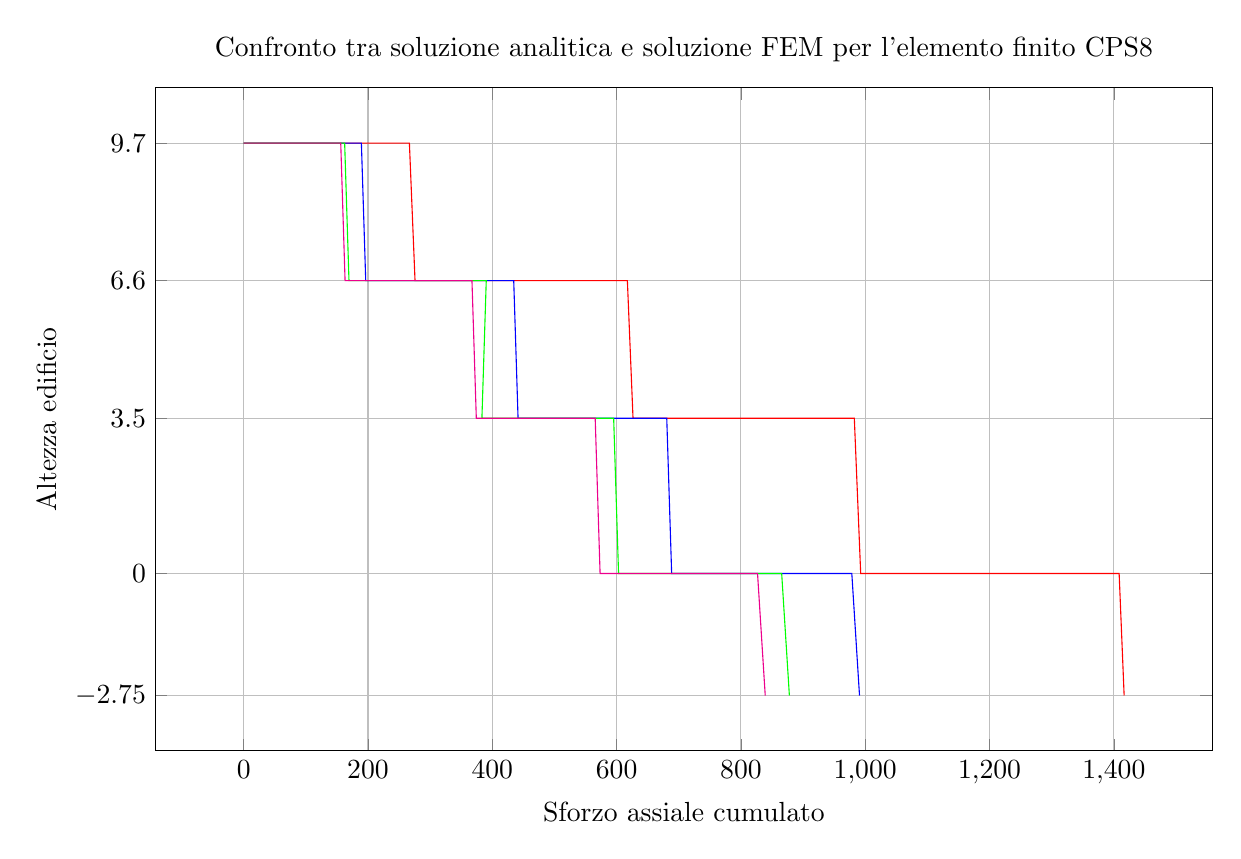
\begin{tikzpicture}\centering
	\begin{axis}[
	    height=10cm,
		width=15cm,
		grid=major,
		xlabel=Sforzo assiale cumulato,
		ylabel=Altezza edificio,
		ytick = {9.7,6.6,3.5,0,-2.75},
		title=Confronto tra soluzione analitica e soluzione FEM per l'elemento finito CPS8
    ]
	\addplot[color=red] coordinates {
	   (0000.00, 9.7  )
	   (0266.64, 9.7  )
	   (0275.70, 6.6  )
	   (0617.34, 6.6  )
	   (0626.41, 3.5  )
	   (0982.45, 3.5  )
	   (0992.69, 0    )
	   (1408.49, 0    )
	   (1416.53, -2.75)
	};
	\addplot[color=blue] coordinates {
	   (0000.00,  9.7  )
	   (0189.40, 9.7  )
	   (0196.37, 6.6  )
	   (0434.48, 6.6  )
	   (0441.45, 3.5  )
	   (0680.68, 3.5  )
	   (0688.56, 0    )
	   (0978.41, 0    )
	   (0990.79, -2.75)
	};
	\addplot[color=green] coordinates {
	   (0000.00,  9.7  )
	   (0162.48, 9.7  )
	   (0169.45, 6.6  )
	   (0390.28, 6.6  )
	   (0383.31, 3.5  )
	   (0595.26, 3.5  )
	   (0603.13, 0    )
	   (0865.58, 0    )
	   (0877.96, -2.75)
	};
	\addplot[color=magenta] coordinates {
	   (0000.00,  9.7  )
	   (0156.17, 9.7  )
	   (0163.15, 6.6  )
	   (0367.30, 6.6  )
	   (0374.28, 3.5  )
	   (0565.55, 3.5  )
	   (0573.42, 0    )
	   (0826.74, 0    )
	   (0839.11, -2.75)
	};
	\end{axis}
\end{tikzpicture}























































































